\documentclass[t]{beamer}
\usepackage[utf8]{inputenc}  % to be able to type unicode text directly
%\usepackage[french]{babel}   % french typographical conventions
\usepackage{inconsolata}     % for a nicer (e.g. non-courier) tt family font
%\usepackage{amsthm,amsmath}  % fancier mathematics
\usepackage{array} % to fine-tune tabular spacing
\usepackage{bbm} % for blackboard 1

\usepackage{graphicx}        % to include images
%\usepackage{animate}         % to include animated images
\usepackage{soul}            % for colored strikethrough
%\usepackage{bbding}          % for Checkmark and XSolidBrush
\usepackage{hyperref,url}

\colorlet{darkgreen}{black!50!green}  % used for page numbers
\definecolor{term}{rgb}{.9,.9,.9}     % used for code insets

\setlength{\parindent}{0em}
\setlength{\parskip}{1em}


% coco's macros
\def\R{\mathbf{R}}
\def\F{\mathcal{F}}
\def\x{\mathbf{x}}
\def\y{\mathbf{y}}
\def\u{\mathbf{u}}
\def\Z{\textbf{Z}}
\def\d{\mathrm{d}}
\DeclareMathOperator*{\argmin}{arg\,min}
\DeclareMathOperator*{\argmax}{arg\,max}
\newcommand{\reference}[1] {{\scriptsize \color{gray}  #1 }}
\newcommand{\referencep}[1] {{\tiny \color{gray}  #1 }}
\newcommand{\unit}[1] {{\tiny \color{gray}  #1 }}

% disable spacing around verbatim
\usepackage{etoolbox}
\makeatletter\preto{\@verbatim}{\topsep=0pt \partopsep=0pt }\makeatother

% disable headings, set slide numbers in green
\mode<all>\setbeamertemplate{navigation symbols}{}
\defbeamertemplate*{footline}{pagecount}{\leavevmode\hfill\color{darkgreen}
   \insertframenumber{} / \inserttotalframenumber\hspace*{2ex}\vskip0pt}

%% select red color for strikethrough
\makeatletter
\newcommand\SoulColor{%
  \let\set@color\beamerorig@set@color
  \let\reset@color\beamerorig@reset@color}
\makeatother
\newcommand<>{\St}[1]{\only#2{\SoulColor\st{#1}}}
\setstcolor{red}

% make everything monospace
\renewcommand*\familydefault{\ttdefault}

%%RUN_VERBATIMS sh
\begin{document}

\addtocounter{framenumber}{-1}
\begin{frame}[plain,fragile]
\LARGE
\begin{verbatim}





  visualization of topographic maps




mnhrdt
gtti 25/5/2022
\end{verbatim}
\end{frame}

\begin{frame}
VISUALIZATION OF TOPOGRAPHIC MAPS\\
=================================

A {\bf topographic map} is a function~$\color{blue}(x,y)\mapsto h(x,y)$
representing the height of a surface.

\vfill

\vfill

{\bf\color{darkgreen} The best way} to visualize a topographic map is
to rotate the 3D surface interactively.
\pause

\fbox{
\fbox{
\fbox{
My goal here is to present {\bf\color{red} the second best} way.
}
}
}
\end{frame}

\begin{frame}[fragile]
VISUALIZATION OF TOPOGRAPHIC MAPS\\
=================================


%lluc meinhardt

\tiny
 \begin{verbatim}
0. History, context
0.1. What is a TM, DEM, DSM, DTM
0.2. History of map colorization
0.3. Fuji 3d photos, identify landmarks
0.4. Rotate 3d model interactively

1. Symbolic-based methods
1.1. Palette (gray, color)
1.2. Level lines
1.3. Level lines + palette (zelda!)
1.4. Slope = closeness of level lines, norm of gradient
1.5. Slope angle = direction of level lines, gradient vector field, grad.-form
1.6. Curvature sign = convexity, concavity of level lines

2. Light-based methods
2.1. Shadows
2.2. Lambertian shading (gouraud, + linear approximation)
2.3. Clear sky shading (ao sampling, + linear approximation)
2.4. Specular shading (phong)
2.5. SAR direct model

3. Uses and fancy things
3.1. To observe defects, understand geometry, etc
3.2. Combined methods: tinted hillshade with level-lines
3.3. As a texture for a 3D rendering
3.4. As a direct model for several famous inverse problems
3.5. Take home message: do not show "north up" in optical images
3.6. Colophon: this document is a notebook
\end{verbatim}

\end{frame}

\begin{frame}
HISTORY, CONTEXT\\
================
\end{frame}

\begin{frame}
What is a TM, DEM, DSM, DTM\\
===========================
\end{frame}

\begin{frame}
History of map colorization\\
================
\end{frame}

\begin{frame}
MODERN CARTOGRAPHY\\
==================

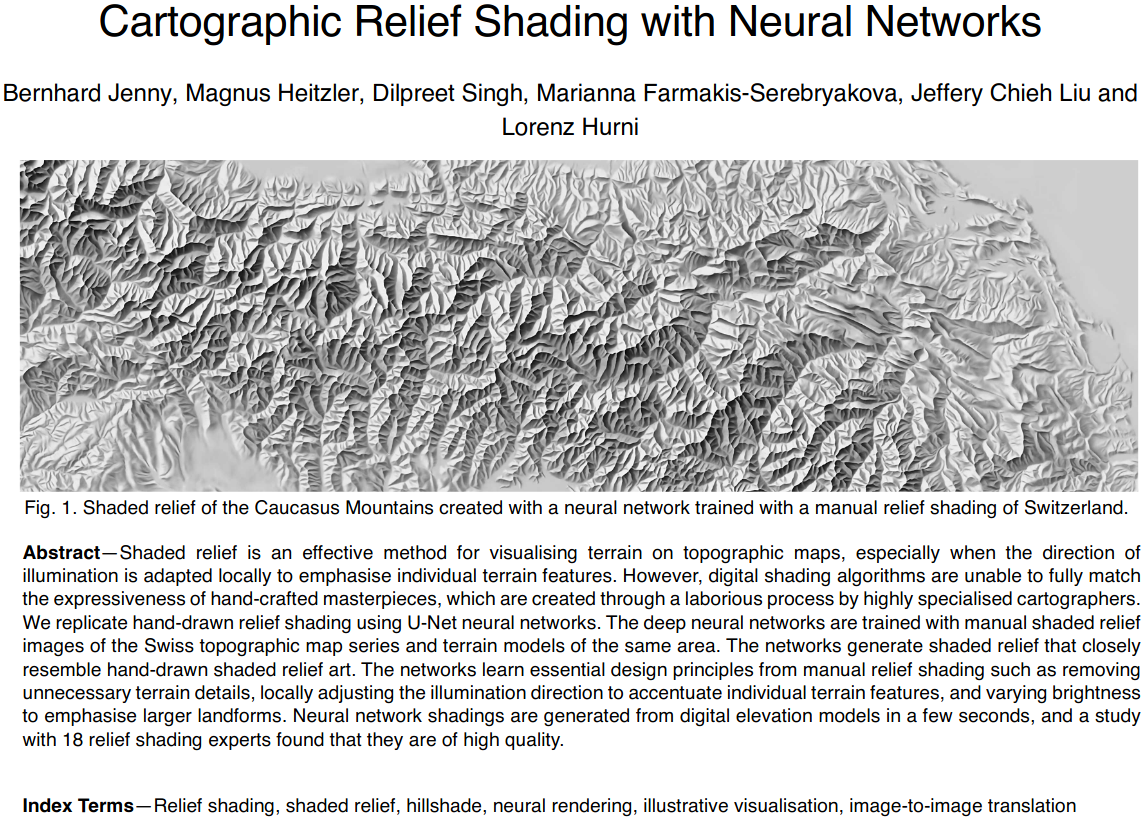
\includegraphics[width=\linewidth]{fs/satire.png}
\end{frame}

\begin{frame}
Fuji 3d photos, identify landmarks\\
================

% https://earth.google.com/web/@35.43358604,138.66641909,1286.03715416a,6726.59176094d,35y,115.23907572h,78.15012473t,0r
\end{frame}

\begin{frame}
Rotate 3d model interactively\\
================
\end{frame}

\begin{frame}
Symbolic-based methods\\
================
\end{frame}

\begin{frame}[fragile]
Palette (gray, color)\\
================

%SCRIPT palette 0 4000 gray f/fuji.npy f/fuji_gray.png -l f/fuji_gray_l.png &
%SCRIPT palette 0 4000 dem f/fuji.npy f/fuji_dem.png -l f/fuji_dem_l.png &
%SCRIPT palette 0 4000 fs/Default.gpl f/fuji.npy f/fuji_def.png -l f/fuji_def_l.png &
%SCRIPT palette 0 4000 botw f/fuji.npy f/fuji_botw.png -l f/fuji_botw_l.png &

%SCRIPT plambda f/fuji.npy "x 270 + 360 / 1 fmod 360 *  1 1 rgb hsv2rgb 255 *"|blur C 1|qauto -i - f/fuji_franges.png &

%SCRIPT plambda f/fuji.npy 'x,n not x 21 < or 255 *'|morsi square opening - f/fuji_water.png
%SCRIPT plambda f/fuji_water.png f/fuji_dem.png "x not y 20 100 255 rgb if" -o f/fuji_dem_water.png &
\only<1>{\includegraphics[width=0.9\textwidth]{f/fuji_gray.png}%
\includegraphics[width=0.1\textwidth]{f/fuji_gray_l.png}}%
\only<2>{\includegraphics[width=0.9\textwidth]{f/fuji_def.png}%
\includegraphics[width=0.1\textwidth]{f/fuji_def_l.png}}%
\only<3>{\includegraphics[width=0.9\textwidth]{f/fuji_franges.png}}
\only<4>{\includegraphics[width=0.9\textwidth]{f/fuji_dem.png}%
\includegraphics[width=0.1\textwidth]{f/fuji_dem_l.png}}%
\only<5>{\includegraphics[width=0.9\textwidth]{f/fuji_dem_water.png}%
\includegraphics[width=0.1\textwidth]{f/fuji_dem_l.png}}%
%\only<6>{\includegraphics[width=0.9\textwidth]{f/fuji_botw.png}%
%\includegraphics[width=0.1\textwidth]{f/fuji_botw_l.png}}%

\end{frame}

\begin{frame}
LEVEL LINES\\
===========

%SCRIPT blur -s l 1 f/fuji.npy f/fuji_b.npy

%SCRIPT echo 1000 500 400 300 200 100 90 80 70 60 50 40 30 20 10|tr ' ' '\n'|while read s; do plambda f/fuji_b.npy "$s >1 <1 / floor <1 *"|morsi cross egradient|plambda '-1 * dup dup rgb'|qauto -p 0|fontu puts 10x20 10 10 "S=$s" -c 800 -b 888 - f/fuji_ll_$s.png ; done &

\only<1>{\includegraphics[width=0.9\textwidth]{f/fuji_ll_1000.png}}%
\only<2>{\includegraphics[width=0.9\textwidth]{f/fuji_ll_500.png}}%
\only<3>{\includegraphics[width=0.9\textwidth]{f/fuji_ll_400.png}}%
\only<4>{\includegraphics[width=0.9\textwidth]{f/fuji_ll_300.png}}%
\only<5>{\includegraphics[width=0.9\textwidth]{f/fuji_ll_200.png}}%
\only<6>{\includegraphics[width=0.9\textwidth]{f/fuji_ll_100.png}}%
%\only<7>{\includegraphics[width=0.9\textwidth]{f/fuji_ll_90.png}}%
%\only<8>{\includegraphics[width=0.9\textwidth]{f/fuji_ll_80.png}}%
%\only<9>{\includegraphics[width=0.9\textwidth]{f/fuji_ll_70.png}}%
%\only<10>{\includegraphics[width=0.9\textwidth]{f/fuji_ll_60.png}}%
%\only<11>{\includegraphics[width=0.9\textwidth]{f/fuji_ll_50.png}}%
%\only<12>{\includegraphics[width=0.9\textwidth]{f/fuji_ll_40.png}}%
%\only<13>{\includegraphics[width=0.9\textwidth]{f/fuji_ll_30.png}}%
%\only<14>{\includegraphics[width=0.9\textwidth]{f/fuji_ll_20.png}}%
%\only<15>{\includegraphics[width=0.9\textwidth]{f/fuji_ll_10.png}}%
\end{frame}

\begin{frame}
LEVEL LINES + PALETTE\\
=====================

%SCRIPT plambda f/fuji_b.npy "200 / round 200 *" -o f/fuji_q.npy
%SCRIPT palette 0 4000 botw f/fuji_q.npy f/fuji_q.png
%SCRIPT morsi cross igradient f/fuji_q.npy | plambda f/fuji_q.png - 'x y not *'|plambda f/fuji_water.png - 'x not y 54 64 70 rgb if'|blur -s l .6|qauto -p 3 -i - f/fuji_zelda.png &
\only<1>{\includegraphics[width=0.9\textwidth]{f/fuji_zelda.png}%
\includegraphics[width=0.1\textwidth]{f/fuji_botw_l.png}}%
\only<2>{\includegraphics[width=0.9\textwidth]{f/fuji_zelda.png}%
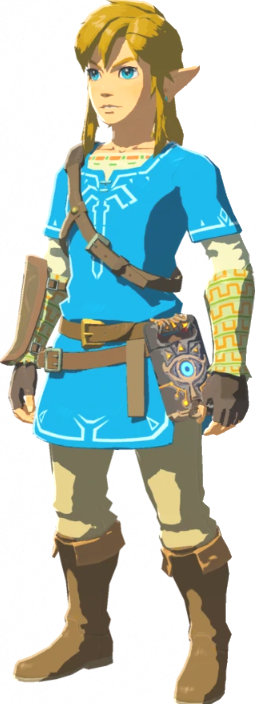
\includegraphics[width=0.1\textwidth]{fs/wlink.png}}%
\end{frame}

\begin{frame}
DENSITY OF LEVEL LINES = SLOPE\\
==============================

%SCRIPT plambda f/fuji_b.npy "x,n -1 *" |qauto -p 0 - f/fuji_slope.png &

\only<1>{\includegraphics[width=0.9\textwidth]{f/fuji_ll_1000.png}$\color{blue}u^{-1}(1000\Z)$}%
\only<2>{\includegraphics[width=0.9\textwidth]{f/fuji_ll_500.png}$\color{blue}u^{-1}(500\Z)$}%
\only<3>{\includegraphics[width=0.9\textwidth]{f/fuji_ll_400.png}$\color{blue}u^{-1}(400\Z)$}%
\only<4>{\includegraphics[width=0.9\textwidth]{f/fuji_ll_300.png}$\color{blue}u^{-1}(300\Z)$}%
\only<5>{\includegraphics[width=0.9\textwidth]{f/fuji_ll_200.png}$\color{blue}u^{-1}(200\Z)$}%
\only<6>{\includegraphics[width=0.9\textwidth]{f/fuji_ll_100.png}$\color{blue}u^{-1}(100\Z)$}%
\only<7>{\includegraphics[width=0.9\textwidth]{f/fuji_ll_90.png}$\color{blue}u^{-1}(90\Z)$}%
\only<8>{\includegraphics[width=0.9\textwidth]{f/fuji_ll_80.png}$\color{blue}u^{-1}(80\Z)$}%
\only<9>{\includegraphics[width=0.9\textwidth]{f/fuji_ll_70.png}$\color{blue}u^{-1}(70\Z)$}%
\only<10>{\includegraphics[width=0.9\textwidth]{f/fuji_ll_60.png}$\color{blue}u^{-1}(60\Z)$}%
\only<11>{\includegraphics[width=0.9\textwidth]{f/fuji_ll_50.png}$\color{blue}u^{-1}(50\Z)$}%
\only<12>{\includegraphics[width=0.9\textwidth]{f/fuji_ll_40.png}$\color{blue}u^{-1}(40\Z)$}%
\only<13>{\includegraphics[width=0.9\textwidth]{f/fuji_ll_30.png}$\color{blue}u^{-1}(30\Z)$}%
\only<14>{\includegraphics[width=0.9\textwidth]{f/fuji_ll_20.png}$\color{blue}u^{-1}(20\Z)$}%
\only<15>{\includegraphics[width=0.9\textwidth]{f/fuji_ll_10.png}$\color{blue}u^{-1}(10\Z)$}%
%\only<16>{\includegraphics[width=0.9\textwidth]{f/fuji_ll_1.png}$\color{blue}u^{-1}(\Z)$}%
\only<16>{\includegraphics[width=0.9\textwidth]{f/fuji_slope.png}$\color{blue}\ \left\|\nabla u\right\|$}%

\end{frame}

\begin{frame}
Slope angle = direction of level lines, gradient vector field, grad.-form\\
================
\end{frame}

\begin{frame}
GRADIENT \hfill{\color{blue}\fbox{$\nabla u = (u_x, u_y)$}}\\
========

%SCRIPT plambda f/fuji_b.npy 'x,g'|flowarrows 2 17 - f/fuji_arrows.png &
%SCRIPT plambda f/fuji_b.npy 'x,g'|viewflow 0 - f/fuji_viewflow.png &
%SCRIPT plambda f/fuji.npy 'x,gf split dup rgb'|qauto -p 1 - f/fuji_grad.png &
%SCRIPT flowarrows .1 23 fs/colorwheel.tiff f/colorwheel_arrows.png &
%SCRIPT viewflow 0 fs/colorwheel.tiff f/colorwheel_viewflow.png &
%SCRIPT plambda fs/colorwheel.tiff "split dup rgb"|qauto -p 0 - f/colorwheel_rgb.png &

\only<1>{\includegraphics[width=0.9\textwidth]{f/fuji_arrows.png}%
\includegraphics[width=0.1\textwidth]{f/colorwheel_arrows.png}\\arrows}%
\only<2>{\includegraphics[width=0.9\textwidth]{f/fuji_viewflow.png}%
\includegraphics[width=0.1\textwidth]{f/colorwheel_viewflow.png}\\colorwheel}%
\only<3>{\includegraphics[width=0.9\textwidth]{f/fuji_grad.png}%
\includegraphics[width=0.1\textwidth]{f/colorwheel_rgb.png}\\RGB=$(u_x,u_y,u_y)$}%

\end{frame}

\begin{frame}
LAPLACIAN \hfill{\color{blue}\fbox{$\Delta u = u_{xx}+ u_{yy}$}}\\
=========

%SCRIPT plambda f/fuji_b.npy 'x,l -1 *'|palette 1% 0 gray - f/fuji_glap.png -l f/fuji_glap_pal.png &
%SCRIPT plambda f/fuji_b.npy 'x,l -1 *'|blur c .5|PLEGEND_REVERSE=1 palette -10 10 nice - f/fuji_lap.png -l f/fuji_lap_pal.png &

\only<1>{
\includegraphics[width=0.9\textwidth]{f/fuji_glap.png}%
\includegraphics[width=0.1\textwidth]{f/fuji_glap_pal.png}
}%
\only<2>{
\includegraphics[width=0.9\textwidth]{f/fuji_lap.png}%
\includegraphics[width=0.1\textwidth]{f/fuji_lap_pal.png}\\
{\color{blue}valleys:$\Delta u\!>\!0\quad$}
{\color{red}ridges:$\Delta u\!<\!0\quad$}
{\color{gray}planar:$\Delta u\!\approx\!0$}}

\end{frame}


\begin{frame}
CURVATURE \hfill{\color{blue}\fbox{$\mathrm{curv}(u)=\mathrm{div}(\nabla u/\|\nabla u\|)$}}\\
=========

%SCRIPT plambda f/fuji.npy 'x,gs dup vnorm /'|plambda 'x,ds -1 *'|PLEGEND_REVERSE=1 palette 1% 0 nice - f/fuji_rcurv.png -l f/fuji_rcurv_pal.png &
%SCRIPT plambda f/fuji_b.npy 'x,gf dup vnorm /'|plambda 'x,db -1 *'|blur c 1|PLEGEND_REVERSE=1 palette -0.2 0.2 nice - f/fuji_curv.png -l f/fuji_curv_pal.png &

\only<1>{
\includegraphics[width=0.9\textwidth]{f/fuji_rcurv.png}%
\includegraphics[width=0.1\textwidth]{f/fuji_rcurv_pal.png}
\small
{\color{blue}valleys:$\mathrm{curv}(u)\!\ge\!0\quad$}
{\color{red}ridges:$\mathrm{curv}(u)\!\le\!0\quad$}
{flat:$\mathrm{curv}(u)=\textrm{NaN}$}
}%
\only<2>{
\includegraphics[width=0.9\textwidth]{f/fuji_curv.png}%
\includegraphics[width=0.1\textwidth]{f/fuji_curv_pal.png}
}
\only<3>{
\includegraphics[width=0.9\textwidth]{fs/fuji_far.jpg}\\
\scriptsize
\color{darkgreen}curvature + retinex kernel (rivers and passes become easier to see)
}

\end{frame}

%\begin{frame}
%Curvature sign = convexity, concavity of level lines\\
%
%================
%\end{frame}

\begin{frame}
LIGHT-BASED METHODS\\
===================

2. Light-based methods\\
2.1. Shadows\\
2.2. Point-source shading (exact, linear approx.)\\
2.3. Cloudy-sky shading (exact, linear approx.)\\
2.4. Specular shading (Phong)\\
2.5. Reflective shading (Oren-Nayar)\\
2.6. SAR direct model\\

\vfill

\includegraphics[width=\linewidth]{fs/brdf.png}\\
\small\color{darkgreen}
different lighting models (for a single light source)

\end{frame}

\begin{frame}
Shadows, shading, reflections\\
=============================

\includegraphics[width=\linewidth]{fs/lighting.jpg}
\end{frame}

\begin{frame}
Shadows\\
================

%SCRIPT plambda f/fuji.npy "10 /" -o f/fuji_p.npy
%SCRIPT shadowcast 0.58 0.81 0    -M f/fuji_p.npy f/fuji_shad1.png &
%SCRIPT shadowcast 0.18 0.26 2.93 -M f/fuji_p.npy f/fuji_shad2.png &

\only<1>{\includegraphics[width=\linewidth]{f/fuji_shad1.png}}%
\only<2>{\includegraphics[width=\linewidth]{f/fuji_shad2.png}}%

\end{frame}

\begin{frame}
Lambertian shading (gouraud, + linear approximation)\\
================
\end{frame}

\begin{frame}
Clear sky shading (ao sampling, + linear approximation)\\
================

%SCRIPT periodize < f/pteri.tif|fft|plambda ':R .7 ^ *'|ifft|imhalve|qeasy -140 40 - f/pteri_linssao.png

%%SCRIPT CX=1; for i in `seq 1 1000`; do SRAND=$i plambda -c "randu randu randu vec 2 * 1 - >1 <1 vnorm 1 > <1 dup vnorm / nan if" ; done|grep -v nan|grep -v '^-'|awk '{print $2 " "  $3 " " $1 }'|while read p q r; do echo shadowcast -M $p $q $r f/pteri.tif /tmp/teri_shey_${CX}.png ; CX=$[CX+1] ; done|parallel -j 8
%SCRIPT veco avg /tmp/teri_shey_* | qauto -p 1 - f/pteri_ao.png
\only<1>{\includegraphics[width=\textwidth]{f/pteri_linssao.png}}%
\only<2>{\includegraphics[width=\textwidth]{f/pteri_ao.png}}%
\end{frame}

\begin{frame}
Specular shading (phong)\\
================
\end{frame}

\begin{frame}
SAR direct model\\
================
\end{frame}

\begin{frame}
Uses and fancy things\\
================
\end{frame}

\begin{frame}
To observe defects, understand geometry, etc\\
================
\end{frame}

\begin{frame}
Combined methods: tinted hillshade with level-lines\\
================
\end{frame}

\begin{frame}
As a direct model for several famous inverse problems\\
================
\end{frame}

\begin{frame}
Take home message: do not show "north up" in optical images\\
================
\end{frame}


\begin{frame}
COLOPHON\\
========

this document is a notebook
\end{frame}


%SCRIPT wait

\end{document}


% vim:sw=2 ts=2 spell spelllang=en:
